\newpage
\section{Marco teórico}

\subsection{Incertidumbre o Margen de Error}

En un proceso de medición la exactitud de los valores obtenidos depende de diversos factores. Una dato medido siempre tendrá cierto de grado de incertidumbre, que puede ser reducida a medida que se corrigen las faltas o errores sistemáticos del proceso. Sin embargo, la incertidumbre nunca llegará a ser nula, ya que existen factores que dentro de ciertos límites no pueden controlarse con anticipación, lo cual hace imposible conocer el valor exacto del dato objetivo. A estos errores en la medición se los conoce como \textit{errores fortuitos}. A pesar de que estos errores no pueden ser corregidos, se puede realizar una serie de mediciones con el objetivo de calcular el valor más probable $x_m$ (tomando el valor medio de la serie), y el \textit{error máximo absoluto} $\Delta x$ (la diferencia entre el valor medio y la medición mas alejada).

\begin{equation}
    x = x_m \pm \Delta x
\end{equation}

En algunos casos, resulta interesante tener una indicador de la calidad de un procesos de medición a partir de su error absoluto. Es por ello que se utiliza el \textit{error relativo} para caracterizar mejor el nivel de exactitud de una medición.

\begin{equation}
\begin{aligned}
    & e = \frac{\Delta x}{x_m}\\
    & e\% = \frac{\Delta x}{x_m} \cdot 100\%
\end{aligned}
\end{equation}

En los instrumentos de medición \textbf{digitales}, la incertidumbre de una medición se suele especificar mediante la suma dos factores, un factor proporcional y un factor fijo. El proporcional es un número que indica el porcentaje de error que tiene una medición, mientras que el factor fijo indica el error con un cierto numero de dígitos de la cifra menos significativa del visor. Por lo tanto, se puede afirmar que el factor proporcional tiene menor peso a medida que el valor medido se acerca a cero, pero el factor fijo tendrá el mismo peso siempre y cuando no se modifique la escala del instrumento y del visor.

\begin{equation}
    error = 0.5\% + 2\;digitos 
\end{equation}

En los instrumentos de medición \textbf{analógicos}, la incertidumbre de una medición se suele especificar utilizando un \textit{índice o clase de exactitud}, que es un tipo de error relativo porcentual asociado a la escala de medición utilizada (valor fiduciario) en el instrumento. Se puede calcular el error máximo absoluto $\Delta x$ de una medición realizando el siguiente cálculo:

\begin{equation}
    \Delta x = \frac{Clase}{100} \cdot Valor fiduciario
\end{equation}

En nuestro país, la norma IRAM - 2039 fija como clase de instrumentos: 

\begin{equation}
    0.25 \;;\; 0.5 \;;\; 1 \;;\; 1.5 \;;\; 2 \;;\; 3 
\end{equation}


\subsection{Medición de cuatro puntos}

El método de medición a cuatro puntas, también conocido como método de Kelvin, es una técnica de medición de impedancia eléctrica que utiliza un voltímetro y un amperímetro para lograr mediciones más exactas de resistencia que al usar la técnica tradicional de medición a dos puntas. El método de medición a cuatro puntas es particularmente útil para la medición de resistencias pequeñas, ya que elimina las contribuciones de las resistencias de cableado y los potenciales de contacto sobre la medición final de la resistencia en cuestión; es por esto que algunos óhmetros de alta precisión se construyen utilizando circuitos similares.

Los problemas de la medición tradicional o a dos puntas (con un ohmetro como el del multímetro) de resistencia, se presentan cuando la resistencia en cuestión es demasiado pequeña. En estos casos, la resistencia del cable de las puntas del multímetro y la resistencia de contacto, ya no son despreciables en comparación con la resistencia a medir, lo que llevaría a una medición errónea.

Es por esto que se emplea este método de cuatro puntas, para lo cual se utilizan un amperímetro y un voltímetro. Entonces, haciendo circular una corriente conocida por la resistencia incógnita, al medir el potencial que cae en la misma y mediante la Ley de Ohm podremos conocer su valor. El circuito quedaría como se muestra a continuación (figura \ref{fig:ej4puntas}):

\begin{figure}[h!]
        \centering        
       \begin{circuitikz} [scale=1,american, transform shape]
\def\scal{1};
\draw (0,-2) to[V,invert] (0,2) to[rmeterwa, t=I, i=$I_{Rp}$] (2,2) to[R, l=$R_{cable}$] (6,2)--(8,2) to[R, l=$R_{prueba}$] (8,-2)--(6,-2) to[R, l=$R_{cable}$] (2,-2)--(0,-2);

\draw (6,2) to[rmeterwa, t=V, v=$V_{Rp}$, o-o] (6,-2);
\end{circuitikz}
        \caption{Circuito para medición de cuatro puntos de una Resistencia}
        \label{fig:ej4puntas}
\end{figure}

\begin{equation}
    R_{prueba}= \cfrac{V_{Rp}}{I_{Rp}}
\end{equation}

Como los voltímetros poseen una resistencia interna muy grande (usualmente, del orden de los 10 M$\Omega$), prácticamente no circula corriente por el circuito interno. Además, la resistencia de los cables uniendo los circuitos es baja, por lo que la caída de tensión sobre estos es despreciable.

Sin embargo, los instrumentos utilizados para estas mediciones de corriente y tensión, también tienen un margen de error o una incertidumbre asociada, la cual deberemos tener en cuenta para el cálculo de la incertidumbre del valor de la resistencia.



\subsection{Medición de Resistencia de Sistemas de Puesta a Tierra}
\label{sec:MTmrspt}


Para comenzar, un sistema de puesta a Tierra es una conexión eléctrica directa de todas las partes metálicas expuestas de una instalación, sin fusibles ni otros sistemas de protección, con uno o varios electrodos (“jabalina” o “malla conductora”) enterrados en el suelo, con objeto de conseguir que en el conjunto de instalaciones, edificios y superficies próximas al terreno, no existan diferencias de potencial peligrosas y que, al mismo tiempo, permita el paso a tierra de las corrientes de defecto o la de descarga de origen atmosférico.

Para lograr este efecto de tener la misma tensión la resistencia del sistema de puesta a tierra debe ser muy baja, idealmente 0$\Omega$. Sin embargo, en la realidad, la resistencia de un sistema de puesta a tierra, consiste en la suma de la resistencia propia del electrodo (la cual es habitualmente de un valor muy bajo) más la resistencia de contacto entre el mismo y la tierra propiamente dicha, la cual puede considerarse como un material electrolítico. Aunque la resistividad del suelo puede ser elevada (y variable dependiendo del tipo de terreno), la resistencia entre dos puntos de conexión a tierra cercanos entre sí puede resultar de un valor muy bajo debido al gran tamaño de la sección transversal del suelo. 

Para poder medir la resistencia real de este sistema, se utiliza el método de 4 puntos descrito anteriormente. El instrumento que se utiliza se conoce como “Telurímetro”, y permite hacer la medición en forma directa. Un Telurímetro moderno consiste en un aparato de medición que contiene un Voltímetro cuya lectura esta calibrada directamente en ohm, y una fuente de corriente constante, que debe ser de corriente alterna de baja frecuencia (no puede ser de corriente continua por los efectos de polarización que se producirían debido a las reacciones electrolíticas). Además, como los Telurímetros se emplean principalmente para medir sistemas de puesta a tierra de redes eléctricas, la frecuencia debe ser diferente de la frecuencia de la red eléctrica y para evitar la interferencia de la red, el voltímetro es selectivo a la frecuencia del generador de corriente.

La medición con este instrumento comúnmente se realiza mediante la inserción de unas sondas metálicas (electrodos) en el suelo, a una distancia determinada de la puesta a tierra, como se puede ver a continuación (figura \ref{fig:circtelurimetro}). 

\begin{figure}[h!]
        \centering        
        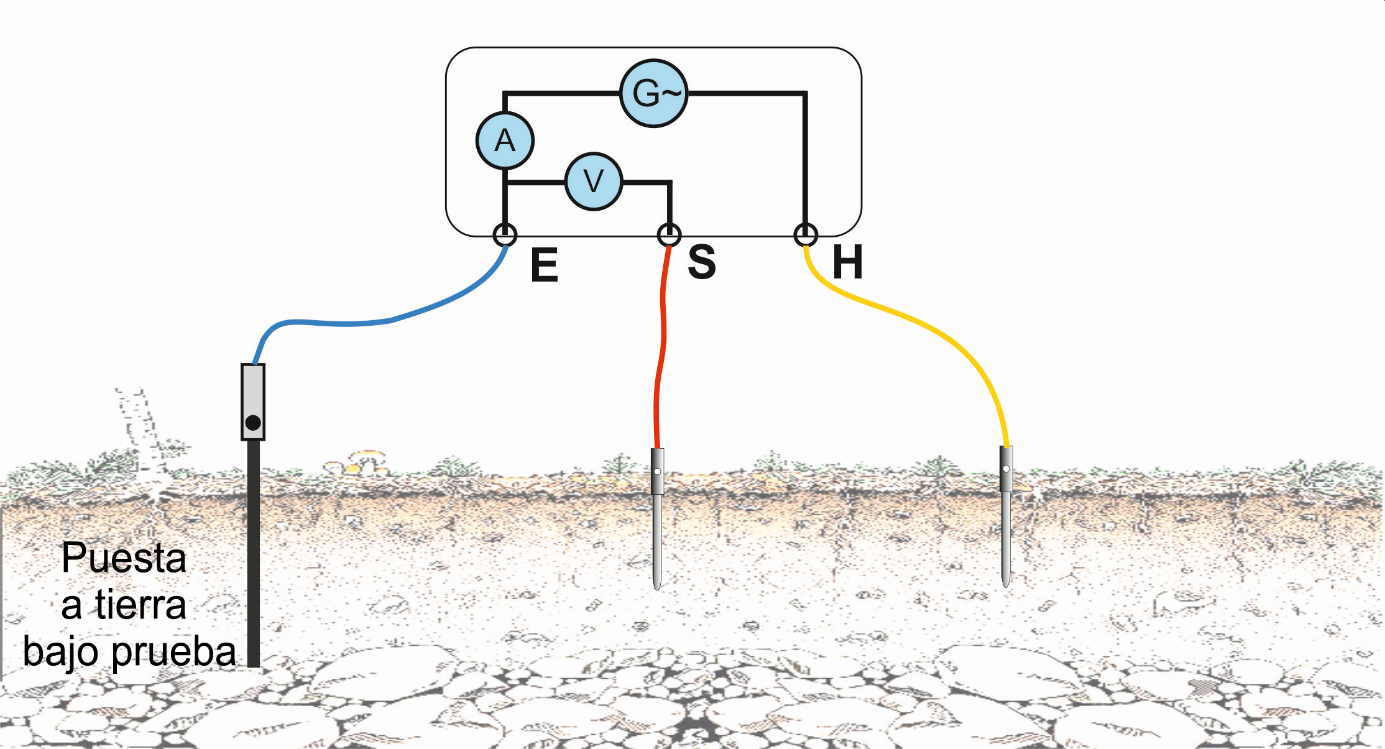
\includegraphics[width=0.6\textwidth]{Imagenes/circTelur.png}
        \caption{Esquema de conexión de un Telurímetro para medición la resistencia de un sistema de puesta a Tierra}
        \label{fig:circtelurimetro}
\end{figure}

Se inserta un electrodo de corriente, que será el encargado de hacer circular la corriente de la fuente y uno de potencial o tensión, que será el que mida el potencial entre la puesta a tierra y ese punto. Internamente y mediante la ley de Ohm, el telurímetro hará el cálculo de la resistencia en este tramo y la mostrará en el visor. 